% !TeX root = ../main.tex
% 原始章节：16-chip-frontend.Rmd

\chapter{芯片前端实现}\label{chap:16-chip-frontend}

\section{需求分析}\label{sec:16-chip-frontend-001}

芯片前端设计的首要步骤是需求分析。
除了技术实现角度的需求，从国产意义的角度来说，如何实现自主产权CPU打破国外CPU技术垄断也是我们国家所亟待解决的问题。

\subsection{从国产意义的角度}\label{sec:16-chip-frontend-002}

目前主流CPU市场被国外垄断，CPU核心技术领域多年来一直落后于国外。而国产CPU的研发和生产，意义深远，主要可体现在以下几个方面：

\begin{itemize}
\tightlist
\item
  提升国家信息安全：国产CPU的研制有助于减少对国外技术的依赖，提高我国信息产业的核心竞争力。特别是在信息安全领域，使用自主可控的CPU可以大大降低被外部势力攻击和监控的风险，保障国家信息安全。
\item
  推动产业升级：国产CPU的研发和生产，将带动整个芯片产业链的发展，包括设计、制造、封装测试等环节，形成良性循环，推动国内芯片产业升级；且CPU是各类电子设备的核心组件，其性能直接关系到设备的整体性能。国产CPU的发展将推动我国电子产品向高性能、低功耗方向发展，满足市场需求，进而带动相关产业的发展。
\item
  增强国际竞争力：随着国产CPU技术的不断成熟和市场份额的扩大，我国在国际芯片领域的影响力也将逐步提升，为我国在国际舞台科技领域上争取更多话语权。
\item
  促进技术创新：国产CPU的研发和生产，将激发我国科技人员的创新活力，推动更多原创性、颠覆性技术的产生。国产CPU的发展需要产学研各方的紧密合作。通过加强产学研合作，可以推动科技成果的转化和应用，提升我国科技产业的整体实力。
\end{itemize}

\subsection{从芯片实现的角度}\label{sec:16-chip-frontend-003}

这一阶段的目的是明确芯片的功能、性能指标、成本目标和市场定位，为后续设计工作奠定基础。需求分析的深度和准确性直接影响到整个项目的成功。
芯片规格制定的主要目标在于明确定义出芯片的功能和性能需求，包括芯片工艺、主频、面积、功耗、存储、IO等，并进行可行性分析，确定需遵守的行业标准和规范。

\subsubsection{功能定位}\label{sec:16-chip-frontend-004}

芯片功能是第一性的，它直接决定了芯片的出发点。对于CPU数字逻辑芯片来说，也有不同的应用场景。比如嵌入式MCU、个人计算机CPU、移动端CPU以及高性能服务器端CPU等。不同的功能定位对于实现功能与性能需求差异很大。比如嵌入式MCU可能更多需要的多外设的需求，而服务器CPU需要非常高的计算能力。

\subsubsection{性能需求}\label{sec:16-chip-frontend-005}

芯片的性能有多个方面综合考量的因素。首先是芯片工艺，先进的工艺节点虽然性能更优，但制造成本也更高，需要根据预算和市场需求来选择合适的工艺节点。对于处理器芯片来说，衡量芯片运算能力的关键指标之一就是时钟频率。一般越精密的工艺所设计制造出来的处理器的主频越高，需要根据具体的应用场景和需求来选择合适的工艺。一般面积、性能、功耗是需要相互权衡的，对于不同的应用场景来说所需要侧重的点不同。比如对于移动端设备需要面积不能太大，功耗不能太高的CPU，而服务器场景下的CPU则更侧重性能。

\subsubsection{技术选型}\label{sec:16-chip-frontend-006}

CPU芯片的设计需要考量使用何种架构、何种总线以及何种存储、IO设置等因素。架构上现代CPU通常采用先进的微架构，如Intel的Skylake、Raptor
Lake或AMD的Zen、Zen
4等。这些架构在指令集、存储结构、分支预测等方面做了优化，以提升处理性能。CPU总线有多种类别，包括内部系统总线以及外部与内存交互的总线等。为了处理内存与CPU之间的处理速度差异，一般CPU都会有缓存进行作为桥梁。现代CPU一般有三级缓存L1、L2、L3
Cache。除了CPU核心的设计，还要考虑整体SOC的设计，以匹配不同的应用需求。

\section{芯片技术规格制定（SPEC）}\label{sec:16-chip-frontend-007}

首先，需要制定芯片的整体架构，包括各功能模块、互连和数据流。这一步骤通常需要硬件工程师和系统架构师的协同工作。
其次，进行性能建模和仿真，使用架构模拟工具进行性能建模和仿真，以验证设计是否符合规格要求，这可以帮助在实际制造之前发现和解决潜在问题。
进而，针对芯片规格进行细化，通过标准代码描述或者文档等形式，制定出各个模块的详细要求，以及与其他系统组件的接口规范。

\subsection{整体功能界定}\label{sec:16-chip-frontend-008}

确定芯片需要集成什么功能。首先一款CPU芯片需要CPU核心与SOC外设与互联设备。对于CPU核心，更多关注在实现性能上，以及存储大小等。而CPU核心以外可以挂接外设以满足多种需求：比如如果需要与外界做网络传输，则需要SOC外设有Ethernet控制器，若需要处理视频数据，则需要JEPG硬解码单元等。而CPU与各个设备之间的互联（即总线）也是设计的重点。

\subsection{架构设计与整体建模}\label{sec:16-chip-frontend-009}

首先要选定指令集架构（ISA），以确保CPU能够高效执行目标应用程序的指令。并且要考虑并行性，考虑如何通过多核、多线程或其他并行计算技术提高性能。如上所述多级缓存设计可以减少内存访问延迟、提高数据访问速度，十分重要。在CPU架构设计中，流水线设计也是需要重点关注的地方，确保指令能够高效地在各个阶段执行，运算资源少闲置。CPU架构设计过程中也要注意模块化设计，这种设计具有可扩展性，允许未来的升级和扩展。除此之外也需要考虑安全性。比如在架构中集成硬件级别的安全特性，如可信执行环境（TEE）、加密引擎等。考虑整体系统集成，确保CPU与内存、I/O设备、外设等硬件之间的接口设计合理。

整体建模主要是为了验证架构设计的合理性与功能的正确性。可以通过System
C等高抽象层级语言编程设计相应架构，再通过原型设计、仿真等方法验证CPU架构的功能正确性。

\subsection{规格细化与文档化}\label{sec:16-chip-frontend-010}

为确保设计团队、开发团队和其他相关人员能够清晰理解芯片的功能、性能、接口和其他关键特性，需要将规格细化以及文档化。以下是如何进行规格细化和文档化的一些内容：

\begin{itemize}
\item
  1.整体概述

  \begin{itemize}
  \tightlist
  \item
    项目背景:
    简要介绍芯片的开发背景，包括目标市场、预期应用、主要客户需求等。
  \item
    设计目标:
    列出芯片的关键设计目标，如性能指标、功耗限制、成本目标、面积约束等。
  \item
    架构概述: 提供芯片的高层架构图，简要描述芯片的主要模块和功能。
  \end{itemize}
\item
  2.功能性规格

  \begin{itemize}
  \tightlist
  \item
    模块功能描述:逐一描述芯片中各个模块的功能，包括处理单元、控制单元、内存控制器、I/O接口等。
  \item
    数据路径与控制逻辑:描述数据在芯片内部的流动路径以及控制逻辑的工作原理。
    操作模式:
  \item
    列出芯片支持的操作模式（如正常模式、节能模式、待机模式等）以及在不同模式下的行为。
  \end{itemize}
\item
  3.性能规格

  \begin{itemize}
  \tightlist
  \item
    计算能力:说明芯片的计算能力，如主频、指令每周期（IPC）、并行度、多核处理能力等。
  \item
    带宽与吞吐量:描述芯片的内存带宽、I/O吞吐量，以及各个接口的最大数据传输速度。
  \item
    时延:详细说明关键操作的时延，包括数据访问、指令执行、缓存命中/未命中等。
  \item
    功耗特性: 列出不同操作模式下的功耗指标，并说明如何进行功耗管理。
  \end{itemize}
\item
  4.接口与引脚定义

  \begin{itemize}
  \tightlist
  \item
    引脚分配:提供芯片引脚的详细分配图，包括每个引脚的功能描述、信号类型（输入/输出）、电气特性等。
  \item
    信号时序:描述重要信号的时序关系，提供时序图表明输入/输出信号之间的依赖关系。
  \item
    接口协议:详细描述芯片支持的接口协议（如SPI、I2C、PCIe、USB等），包括通信协议、数据格式、握手信号等。
  \end{itemize}
\item
  5.物理与电气规格

  \begin{itemize}
  \tightlist
  \item
    封装类型:说明芯片的封装类型和尺寸，以及与电路板的物理连接方式。
  \item
    电气参数:列出芯片的工作电压范围、电流消耗、功率消耗、输入/输出电压特性等。
  \item
    热管理: 提供热设计功耗（TDP）以及推荐的散热解决方案。
  \end{itemize}
\item
  6.测试与验证要求

  \begin{itemize}
  \tightlist
  \item
    测试模式:描述芯片的各种测试模式和相应的测试接口，以支持制造测试和功能验证。
  \item
    验证标准:
    说明芯片在各个功能模块的验证标准，确保设计符合规格要求。
  \item
    测试覆盖率: 列出芯片在各个操作模式和功能状态下的测试覆盖率要求。
  \end{itemize}
\item
  7.软件与工具支持 开发工具链:

  \begin{itemize}
  \tightlist
  \item
    列出芯片支持的开发工具，包括编译器、调试器、仿真工具等。
  \item
    软件库:说明芯片附带的软件库或驱动程序，以及开发环境的支持情况。
  \item
    固件要求:如果芯片需要固件支持，详细说明固件的功能、接口和更新机制。
  \end{itemize}
\end{itemize}

\section{模块级RTL设计实现}\label{sec:16-chip-frontend-011}

在 CPU 设计中，RTL（Register Transfer
Level，寄存器传输级）模块化设计是一种重要的设计方法。它将复杂的 CPU
功能分解为多个相对独立的模块，每个模块实现特定的功能，然后通过合理的连接和交互实现整个
CPU
的功能。这种设计方法具有提高设计效率、增强可维护性、便于验证和调试等优点。

在本教材中，具体的电路架构设计过程参考第四至第十一章，较为全面的讲述了从LA32R指令集开发流程、系统支持到具体的简单CPU设计、进阶CPU设计以及总线、SOC集成、仿真等各个部分，这里主要针对CPU设计中的RTL模块化设计方法进行介绍。需要注意的是本教材的一些地方采用chisel语言实现，chisel语言可以描述RTL代码，通过编译可以生成verilog等可被EDA工具综合的硬件描述。

\subsection{RTL模块化设计基本原则}\label{sec:16-chip-frontend-012}

\begin{itemize}
\item
  1.高内聚低耦合

  \begin{itemize}
  \tightlist
  \item
    每个模块应具有明确的功能边界，内部的逻辑紧密相关，实现高内聚。这样可以使模块的功能更加清晰，便于理解和维护。
  \item
    模块之间的连接应尽量简单，减少不必要的依赖关系，实现低耦合。这样可以降低模块之间的相互影响，提高系统的稳定性和可扩展性。
  \end{itemize}
\item
  2.可重用性

  \begin{itemize}
  \tightlist
  \item
    设计模块时应考虑其可重用性，尽量使模块具有通用性和灵活性。这样可以在不同的项目中重复使用这些模块，提高设计效率，降低开发成本。
  \end{itemize}
\item
  3.易于验证和调试

  \begin{itemize}
  \tightlist
  \item
    模块的设计应便于验证和调试。可以采用一些验证方法，如功能仿真、形式验证等，确保模块的功能正确性。同时，模块的内部结构应尽量简单明了，便于调试和故障排除。
  \end{itemize}
\end{itemize}

\subsection{RTL模块的划分}\label{sec:16-chip-frontend-013}

这里主要介绍对于CPU核的一些RTL模块划分：

\begin{itemize}
\item
  1.控制器模块：负责 CPU
  的指令译码、控制信号生成等功能。它根据指令的类型和操作码，生成相应的控制信号，控制各个模块的操作。
\item
  2.运算器模块：实现 CPU
  的算术运算和逻辑运算功能。它可以进行加法、减法、乘法、除法等算术运算，以及与、或、非等逻辑运算。
\item
  3.寄存器模块：用于存储 CPU
  内部的数据和指令。它可以分为通用寄存器、特殊寄存器等不同类型，根据需要进行读写操作。
\item
  4.存储器模块：存储 CPU
  运行时所需的数据和指令。它可以分为程序存储器和数据存储器，分别用于存储程序和数据。
\item
  5.总线模块：连接各个模块，实现数据和控制信号的传输。它可以分为地址总线、数据总线和控制总线，分别用于传输地址、数据和控制信号。
\end{itemize}

\subsection{RTL模块的设计方法}\label{sec:16-chip-frontend-014}

\begin{itemize}
\item
  1.自顶向下设计：首先从系统的整体功能出发，进行高层次的设计规划。然后逐步将系统分解为多个模块，进行详细的设计和实现。这种设计方法可以使设计人员更好地理解系统的整体结构和功能，提高设计的准确性和效率。
\item
  2.自底向上设计：首先从各个模块的功能出发，进行详细的设计和实现。然后将这些模块组合起来，实现整个系统的功能。这种设计方法可以使设计人员更好地掌握每个模块的细节，提高模块的质量和可靠性。
\item
  3.混合设计：结合自顶向下和自底向上的设计方法，进行系统的设计和实现。在设计过程中，可以根据实际情况灵活选择不同的设计方法，以提高设计的效率和质量。
\end{itemize}

\subsection{RTL模块间的连接与交互}\label{sec:16-chip-frontend-015}

\begin{itemize}
\item
  1.模块之间的连接：模块之间的连接可以通过总线、信号线等方式实现。在连接时，应注意信号的类型、宽度和方向，确保信号的正确传输。
\item
  2.模块之间的交互：模块之间的交互可以通过控制信号、数据信号等方式实现。在交互时，应注意信号的同步和时序关系，确保模块之间的正确协作。
\end{itemize}

\subsection{RTL模块化设计的验证和调试}\label{sec:16-chip-frontend-016}

\begin{itemize}
\item
  1.功能仿真：使用仿真工具对 RTL
  设计进行功能仿真，验证各个模块的功能正确性。可以编写测试用例，对模块的输入输出进行测试，检查模块的功能是否符合设计要求。
\item
  2.形式验证：使用形式验证工具对 RTL
  设计进行形式验证，验证模块的逻辑正确性。形式验证可以检查模块的逻辑是否存在错误，如死锁、活锁等问题。
\item
  3.调试方法：在设计过程中，可以使用调试工具对 RTL
  设计进行调试。调试工具可以帮助设计人员观察模块的内部状态、信号的变化等，便于发现和解决问题。
\end{itemize}

RTL 模块化设计是 CPU
设计中的一种重要方法，它可以提高设计效率、增强可维护性、便于验证和调试。在设计过程中，应遵循高内聚低耦合、可重用性、易于验证和调试等基本原则，合理划分模块，采用合适的设计方法，进行模块的连接和交互，并进行充分的验证和调试，以确保设计的正确性和可靠性。

\section{功能仿真验证}\label{sec:16-chip-frontend-017}

功能仿真即需要通过仿真来验证电路设计在逻辑和功能层面是否满足要求。在本教材3.2.3小节中，简要描述了一小部分功能仿真的环境以及策略。本节将针对功能仿真具体的过程进行描述。

首先需要编写testbench，testbench是用于验证和测试设计中硬件描述语言（HDL）模块或整个系统的环境。testbench模拟设计的操作，生成输入信号，并检查输出是否符合预期，从而确保设计在实际硬件上工作前的正确性。testbench通常与设计单元（如Verilog或VHDL模块）一起编写，并在仿真工具中执行。编写testbench一般流程为：

\begin{itemize}
\item
  1.环境初始化：在开始仿真之前，testbench首先对所有信号进行初始化。这通常包括将所有寄存器和线初始化为已知的默认状态（如零或无效状态）。
\item
  2.信号生成（激励）：testbench通过生成特定的输入信号序列来驱动设计单元。这些输入信号可以是简单的固定模式，也可以是复杂的时序信号或随机信号，视测试需求而定。
\item
  3.设计模块实例化：testbench中实例化被测模块（待测设计DUT），并将生成的输入信号施加到模块的输入端口。
\item
  4.响应检测：一般testbench会检测需要重点关注的DUT输出信号，并将输出信号与预期结果进行对比。这一步通过``检测器''完成。
\item
  5.结果验证：通过检测模块的输出是否符合预期来检测可能存在的错误。
\item
  6.dump波形或打印信息：在对应关键输出结果时，会通过系统函数打印出``正确''或``错误''标志；通过dump波形文件，查看波形来进一步获取信号的变化情况。
\end{itemize}

电路功能仿真除了上述基本的流程以外，还有一些高阶的用法：

\begin{itemize}
\item
  1.自检机制：高级testbench通常具备自检功能，即testbench可以自动检查DUT的输出并决定测试是否通过。这种机制减少了人为干预，提高了测试效率。自检机制通常包括断言（assertions）、覆盖率分析和自动错误报告。
\item
  2.随机化测试：为了提高测试覆盖率，testbench可以使用随机化技术生成输入信号。这种方法可以揭示设计中的边缘情况和罕见错误。随机化测试通常结合约束随机化（constrained
  randomization），以确保输入信号符合设计规范。
\item
  3.基于事务的验证
  (TBA)：TBA是一种高级验证方法，testbench通过模拟系统级事务（如数据包传输、存储器访问等）来测试DUT。这种方法特别适用于复杂的SoC（系统级芯片）验证，能够有效地测试模块之间的交互行为。
\item
  4.功能覆盖率：testbench可以通过功能覆盖率分析来衡量测试的全面性。功能覆盖率分析帮助验证工程师识别未被测试到的设计路径或功能，并引导进一步的测试开发。
\item
  5.UVM (Universal Verification
  Methodology)：UVM是一个行业标准的高级验证框架，使用面向对象的SystemVerilog语言编写。UVM提供了标准化的验证组件、环境和测试用例结构，适用于大规模复杂系统的验证。通过UVM，testbench可以实现模块化、可重用、可扩展的验证环境。
\item
  6.混合级别仿真：在复杂系统中，testbench可以结合不同抽象级别的仿真（如行为级、门级和寄存器传输级）来进行验证。这种混合仿真技术能够在更高的抽象级别快速验证系统行为，同时在较低级别上捕获更多细节。
\end{itemize}

下面给出一个简单的testbench模板，以作教学使用：

% 代码语言：BookVerilog
\begin{CodeBlock}[language=BookVerilog]
// 仿真单位和精度
`timescale 1ns/1ps

// 定义模块与模块名
module simple_tb;

  // DUT参数设置
  parameter WIDTH = 8;

  // 信号描述
  reg clk;
  reg rst_n;
  reg [WIDTH-1:0] data_in;
  wire [WIDTH-1:0] data_out;

  // 实例化 DUT (Device Under Test)
  dut #(
    .WIDTH(WIDTH)
  ) dut_inst (
    .clk(clk),
    .rst_n(rst_n),
    .data_in(data_in),
    .data_out(data_out)
  );

  // 产生时钟
  initial begin
    clk = 0;
    forever #5 clk = ~clk;  // 10ns clock period
  end

  // 产生复位信号
  initial begin
    rst_n = 0;
    #15 rst_n = 1;  // 15ns后释放复位信号
  end

  // 产生激励信号
  initial begin
    // 施加初始值
    data_in = 0;

    // 等待复位取消
    @(posedge rst_n);

    // 施加测试向量
    #10 data_in = 8'hA5;  // 测试向量1
    #10 data_in = 8'h3C;  // 测试向量2
    #10 data_in = 8'hFF;  // 测试向量3

    // 结束仿真
    #50 $finish;
  end

  // 检测DUT输出
  initial begin
    $monitor("Time: %0t | data_in: %0h | data_out: %0h", $time, data_in, data_out);
  end

endmodule
\end{CodeBlock}

其中\$monitor是检测信号系统函数，主要功能为实时显示信号的变化，即在data\_in或者data\_out信号变化时，会打印对应的数据。

在编写完testbench之后使用仿真EDA工具VCS或ModelSim等来进行编译与仿真（具体的工具使用参考15.2节）。

\section{逻辑综合}\label{sec:16-chip-frontend-018}

逻辑综合是芯片前端设计中的一个关键步骤，其作用是逻辑综合是基于特定的工艺库，设定电路的面积、时序等目标参数的约束条件，将设计的RTL级代码映射为门级网表的过程。这一过程旨在决定电路的门级结构，寻求时序与面积的平衡，以及功耗与时序的平衡，同时增强电路的测试性。通过逻辑综合，设计师能够确保设计的功能在物理层面上得到实现，并为后续的布图和后端设计提供基础。

在15.2章节中，简单描述了Synopsys DC综合工具的使用，这里做一个详细展开。

\subsection{逻辑综合概述}\label{sec:16-chip-frontend-019}

逻辑综合过程中，EDA工具会将电路划分成7个处理对象，如图\ref{fig:dc-obj}所示：

\begin{itemize}
\tightlist
\item
  Design：整个需要综合的电路，即我们需要综合的电路设计（RTL）
\item
  Port：最外部的端口，一般是电路与外部交互的IO口
\item
  Clock：由于时钟上的任何问题都会对电路造成重要的影响，所以时钟需要单独处理
\item
  Cell：被例化的模块
\item
  Reference：例化模块的原电路
\item
  Pin：Cell自身的引脚，注意与Port的区别
\item
  Net：内部连线
\end{itemize}

\begin{figure}[htbp]
  \centering
  
\includegraphics[width=0.5\linewidth]{assets/16/DC处理对象划分.png}
  \caption{DC处理对象划分}
  \label{fig:dc-obj}
\end{figure}

逻辑综合通常包括translation、optimization和mapping三个步骤：

\begin{itemize}
\tightlist
\item
  translation：将HDL描述的电路转换为用GTECH库元件组成的逻辑电路，GTECH库是synopsys的通用工艺库，仅表示逻辑函数的功能，并没有映射到具体的厂家工艺库。
\item
  optimization：在这一步骤中，逻辑综合工具会根据设计指标（如时序、面积、功耗等）对转译后的数据库进行优化。优化过程可能会去除一些被认为是``无用的模块''，如未连接的端口或永远不会触发的状态机跳转条件。
\item
  mapping：将优化后的电路转换为目标工艺库对应的门级网表。它确保了电路能够在特定的工艺条件下实现。
\end{itemize}

如图\ref{fig:dc-flow}是Synopsys DC综合工作流程示意图：

\begin{figure}[htbp]
  \centering
  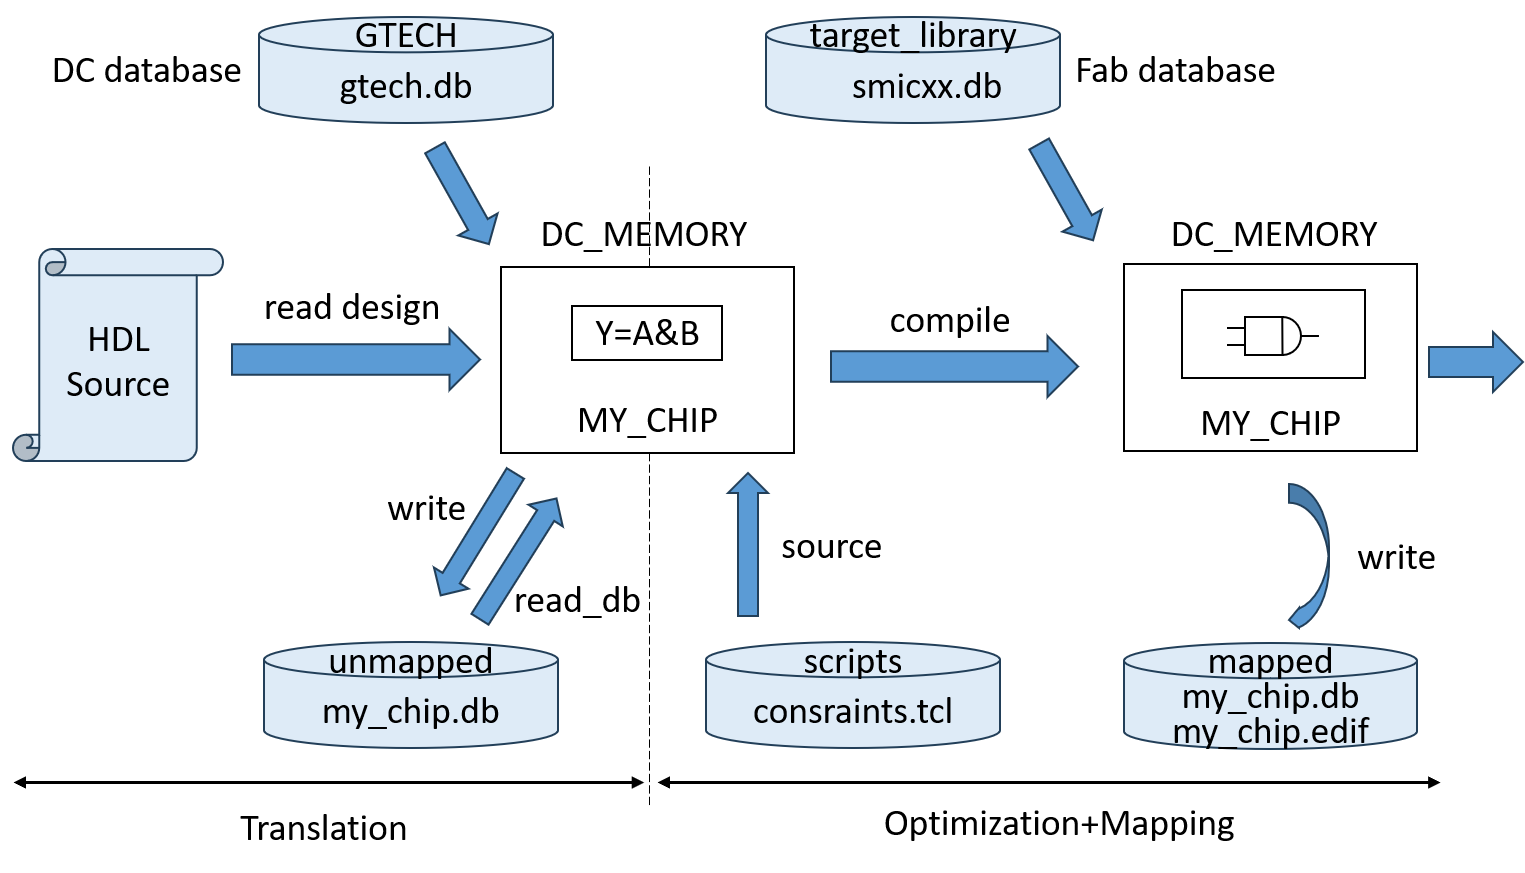
\includegraphics[width=0.5\linewidth]{assets/16/DC综合过程示意图.png}
  \caption{DC综合过程示意图}
  \label{fig:dc-flow}
\end{figure}

\subsection{逻辑综合实施流程}\label{sec:16-chip-frontend-020}

逻辑综合的具体实现流程如图\ref{fig:dc-workflow}所示，包含指定工艺库、读入设计、定义设计环境、设计约束、设计规则约束、优化约束、编译策略选择、分析报告、写文件等过程。下面将针对每一步的设置进行展开描述。

\begin{figure}[htbp]
  \centering
  
\includegraphics[width=0.5\linewidth]{assets/16/DC工作流程.png}
  \caption{DC工作流程}
  \label{fig:dc-workflow}
\end{figure}

\begin{itemize}
\item
  1.设计实现HDL文件：即在综合开始前需要准备好设计完善的可综合RTL文件。
\item
  2.指定库文件：库文件包括链接库（Link library）、目标库（target
  library）、符号库（symbol library）、综合库（synthetic
  library）。其中链接库与目标库是必须指定的，这两者也被称为工艺库，二者可以使用一个库文件。下面对这几种库文件进行描述：

  \begin{itemize}
  \tightlist
  \item
    链接库：用于指定综合工具在解析设计时用来解析逻辑单元的库。这些库文件包含了设计中的所有单元（如门、触发器、宏单元等）的定义。它确保综合过程中引用的所有单元都能被正确解析并链接。
  \item
    目标库：用于指定综合过程中实际进行逻辑映射和优化所使用的库。这些库文件提供了目标单元的时序、功耗、面积等详细信息，Design
    Compiler 将设计映射到这些单元上，并根据它们的特性进行优化。
  \item
    符号库：提供 Design Vision GUI
    中设计实现的图形符号，如果使用脚本模式而不使用
    GUI,此库可不指定。
  \item
    综合库：亦称为 Designware
    库，尽管其名称翻译为``综合库''，但通常被称为 IP 库。某些特殊的
    Designware
    库（例如多级流水线乘法器）需要获得授权许可。然而，默认的标准
    Designware 库由 Design Compiler
    软件供应商直接提供，无需用户额外指定。
  \end{itemize}

  需要注意的是当读入的文件是门级网表时，需要把 link library
  指向生成该门级网表的库文件，否则 DC
  因不知道网表中门单元电路的功能而报错。

  一般设置脚本为：

% 代码语言：BookTcl
\begin{CodeBlock}[language=BookTcl]
set link_library [list "std_cells.db" "macros.db" "black_boxes.db"]
set target_library [list "std_cells.db"]
set symbol_library [list "sym.db"]
set synthetic_library [list "dw_foundation.sldb"]
\end{CodeBlock}
\item
  3.读入设计：设计的读取过程包括将设计文件加载到内存中，并将其转换为
  DC 的中间格式，即 GTECH 格式。GTECH 格式由 `soft macros'
  组成，如加法器、比较器等，这些组件来源于 Synopsys
  的合成库，每种组件有多种不同的结构。读入设计有两种实现方式：

  \begin{itemize}
  \tightlist
  \item
    read\_verilog/read\_vhdl
  \item
    analyze \& elaborate
  \end{itemize}

  第二种读取方式可以自由指定设计库，并在生成GTECH中间文件前生成.syn文件存储于work目录下。这样可以在下次elaborate时节省时间。我们在读取RTL设计时一般选用第二种方法读取。下面是一个使用脚本，其中RTL\_SRC定义了所有源文件路径，ACTIVE\_DESIGN是顶层模块的名称。
\end{itemize}

% 代码语言：BookTcl
\begin{CodeBlock}[language=BookTcl]
analyze -format sverilog $RTL_SRC
elaborate $ACTIVE_DESIGN
link
uniquify
check_design > ./check_design.log
\end{CodeBlock}

\begin{itemize}
\item
  4.定义设计环境：具体包括工艺库的工艺电压温度（PVT）条件、线负载模型、IO端口属性（驱动、扇出、负载等），这些设计环境会影响综合及优化结果。下面给出一些常用命令：

  \begin{itemize}
  \item
    set\_operating\_conditions:指定不同的分析类型（如最坏情况、最好情况或基于芯片变异性的分析），并可以选择不同的库文件（如最慢库、典型库、最快库）来适应不同的分析需求。此外，该指令还可以与其他SDC（Synopsys
    Design
    Constraints）命令结合使用，以更精确地控制设计的时序和功耗特性。
  \item
    set\_driving\_cell/set\_drive/set\_input\_transition：三个命令都会影响输入端口驱动强度。我们通过set\_driving\_cell命令来设置某个输入端口前面是什么驱动单元驱动它的，EDA工具会从指定的库中查找得出更加真实的Transition时间来代替零Transition。set\_drive命令通过为输入端口指定电阻值的方法来为其定义外部驱动强度。在逻辑综合工具进行优化期间，工具根据设置的驱动强度来计算由该输入端口驱动的逻辑电路的延迟。set\_input\_transition命令为输入端口指定一个固定的transition时间，工具会用该transition时间来计算它驱动的逻辑电路的延迟。
  \item
    set\_wire\_load\_model：指定估算线延迟时所选用的模型。包含zero wire
    load model、基于fanout的传统WLM以及基于物理位置的wire load
    model。
  \end{itemize}
\item
  5.设计约束：包括设计规则约束与优化约束。设计规则约束（DRC）由工艺库决定，包括最大转换时间、最大扇出以及最大电容。优化约束就包括关键的时钟约束、输入输出延时以及面积约束等。DC会根据这个优化约束条件来权衡综合出的网表，使之尽量满足约束条件。下面是一些常用的脚本命令：
\end{itemize}

% 代码语言：BookTcl
\begin{CodeBlock}[language=BookTcl]
# 设置最大信号转换时间  
set_max_transition 0.5 -net [get_nets clk_net]  
# 解释：为名为clk_net的网络设置最大信号转换时间为0.5纳秒。这有助于控制信号完整性
  
# 设置最大扇出数  
set_max_fanout 10 -cell BUF_X1  
# 解释：为单元BUF_X1设置最大扇出数为10。这有助于防止由于过多负载而导致的性能下降
  
# 注意：有些工具可能不支持直接为单元设置最大扇出数，而是需要设置最大负载电容等
  
# 设置最大电容值  
set_max_capacitance 0.1 -net data_net  
# 解释：为名为data_net的网络设置最大电容值为0.1皮法。这有助于控制信号延迟和功耗
  
# 创建时钟  
create_clock -name clk -period 10 -waveform {0 5} [get_ports clk_port]  
# 解释：创建一个名为clk的时钟，周期为10纳秒，波形为占空比50%（从0到5纳秒为高电平），并将其
# 与名为clk_port的端口相关联  
  
# 设置时钟延迟  
set_clock_latency 1.0 -source -max [get_clocks clk]  
# 解释：为名为clk的时钟设置源端最大延迟为1.0纳秒。这考虑了时钟源到设计中各点的传播延迟
  
# 设置传播时钟  
set_propagated_clock [get_clocks -of [get_cells buf_inst]]  
# 解释：这通常不是直接设置的命令，而是用于识别和传播时钟的。上面的命令是假设性的，具体取决
# 于工具如何自动处理时钟的传播  
  
# 设置时钟不确定性  
set_clock_uncertainty 0.2 -setup [get_clocks clk]  
# 解释：为名为clk的时钟设置建立时间不确定性为0.2纳秒。这考虑了时钟抖动和其他不确定因素
  
# 设置时钟转换时间  
set_clock_transition 0.3 -clock clk  
# 解释：为名为clk的时钟设置最大转换时间为0.3纳秒。这有助于控制时钟信号的完整性
  
# 设置输入延迟  
set_input_delay -clock clk -max 2.0 [get_ports data_in]  
# 解释：为名为data_in的输入端口设置相对于名为clk的时钟的最大输入延迟为2.0纳秒
#（用于建立时间分析）  
  
# 设置输出延迟  
set_output_delay -clock clk -max 2.5 [get_ports data_out]  
# 解释：为名为data_out的输出端口设置相对于名为clk的时钟的最大输出延迟为2.5纳秒
#（用于保持时间分析）  
  
# 注意：设置最大面积（set_max_area）通常不是时序分析的一部分，而是优化或物理实现阶段可能考虑的约束  
# 假设存在一个设置面积约束的命令，它可能看起来像这样（但具体取决于工具）：  
# set_max_area 1000000 -design my_design  
# 解释：为名为my_design的设计设置最大面积为1000000平方微米
\end{CodeBlock}

\begin{itemize}
\item
  6.选择编译策略：两种编译策略：Top-down与Bottom-up；这两种策略侧重点有所不同：

  \begin{itemize}
  \tightlist
  \item
    Top-down（自顶向下）：适用于小型或中等规模设计，因为这种策略可以再整个设计中应用统一的约束和优化。
  \item
    Bottom-up（自底向上）：适用于大型或非常复杂的设计，因为这种策略运算分阶段编译和优化。
  \end{itemize}

  在使用命令编译时，直接输入compile或compile\_ultra即可编译（是一个更高级的综合命令，用于执行更深层次的优化。它在综合过程中使用了更激进的优化策略，以获得更好的时序、功耗和面积优化）。
\item
  7.分析与报告：report面积（资源）、时序、功耗等信息，查看时序是否收敛、面积是否查出目标范围等。对于设计中存在的问题可以使用check\_design命令来检查。
\item
  8.写网表等文件：在DC结束编译后，可以通过下述命令来实现写网表文件（除了.v格式还有DC支持的.ddc格式）：
\end{itemize}

% 代码语言：BookTcl
\begin{CodeBlock}[language=BookTcl]
write -format verilog -hierarchical -output your_design_synth.v
write -format ddc -hierarchical -output your_design_synth.ddc
\end{CodeBlock}

\section{静态时序分析}\label{sec:16-chip-frontend-021}

静态时序分析（Static Timing Analysis,
STA）是数字集成电路设计中关键的验证步骤，用于确保设计在指定的工作频率下满足所有时序约束。相比动态仿真，STA不依赖特定的输入激励，而是通过分析电路中所有可能的时序路径来验证设计的时序完整性，从而在较短时间内覆盖整个电路。

\subsection{时序路径与基本概念}\label{sec:16-chip-frontend-022}

\begin{itemize}
\item
  时序路径：STA中，路径通常由起点（如触发器的输出端）、组合逻辑电路、和终点（如另一个触发器的输入端）组成。STA分析中，有四种时序路径：

  \begin{itemize}
  \tightlist
  \item
    输入端口到触发器的输入端
  \item
    输入端口到输出端口
  \item
    触发器的时钟到另一个触发器的输入端
  \item
    触发器的时钟到输出端口
  \end{itemize}
\item
  时钟域：时钟域是电路中受同一时钟信号控制的部分。在不同的时钟域之间传递信号可能会引发跨时钟域的问题，因此需要特别关注。
\item
  建立时间（setup）和保持时间（hold）：寄存器对输入信号的要求，即信号必须在时钟边沿前保持稳定（建立时间）并在之后维持一段时间（保持时间）才能被正确采样。如图\ref{fig:setup-hold}所示为概念图。

  \begin{itemize}
  \tightlist
  \item
    建立时间（setup
    time）：寄存器在时钟上升沿到达前应当保持数据不变的时间。
  \item
    保持时间（hold
    time）：寄存器时钟上升沿到达后数据应当继续保持的最短时间。
  \end{itemize}
\end{itemize}

\begin{figure}[htbp]
  \centering
  
\includegraphics[width=0.5\linewidth]{assets/16/建立时间与保持时间概念.png}
  \caption{建立时间与保持时间}
  \label{fig:setup-hold}
\end{figure}

\subsection{静态时序分析的核心步骤}\label{sec:16-chip-frontend-023}

时钟树综合（Clock Tree Synthesis,
CTS）：生成并优化电路中的时钟树，确保时钟信号在所有寄存器中同步到达。时钟树的设计和优化对时序分析的准确性至关重要。

时序约束设置：使用SDC（Synopsys Design
Constraints）文件定义设计的时序约束，包括时钟定义、输入输出延迟、时钟不确定性等。合理的约束设置是STA成功的基础。

路径延迟计算：STA工具通过计算时序路径中的信号传播延迟，包括组合逻辑延迟、寄生效应引起的延迟和时钟延迟，来确定路径是否满足时序约束。

时序违规检测：STA工具会检测是否存在路径延迟超过时钟周期导致的时序违规，并报告潜在的建立时间和保持时间问题。

\subsection{STA中的关键问题}\label{sec:16-chip-frontend-024}

时钟偏斜（Clock
Skew）：由于时钟网络中不同寄存器的时钟到达时间不同，可能引发时序违规。优化时钟偏斜是确保时序正确性的关键。

时钟不确定性（Clock
Uncertainty）：制造工艺差异、温度变化和电源噪声可能导致时钟信号不确定性。STA中需要考虑时钟不确定性，确保时序裕量充足。

多周期路径（Multicycle Paths,
MCP）：一些时序路径需要多个时钟周期才能完成信号传播。STA工具必须正确识别这些路径，避免错误报告时序违规。

假路径（False
Paths）：由于设计原因不会被实际激活的路径应标识为假路径，以防止它们在STA中引发虚假时序违规。

跨时钟域路径（Cross-Clock Domain
Paths）：信号跨越不同时钟域时可能产生时序问题，通常通过同步器或异步FIFO处理。

\subsection{时序优化与收敛}\label{sec:16-chip-frontend-025}

逻辑优化：如果发现时序违规，可以通过重构逻辑路径、减少逻辑级数或插入缓冲器来优化电路。

时钟树优化：通过减少时钟偏斜和抖动来优化时钟树，确保时钟信号在电路中同步分布。

寄生效应优化：调整布局布线以减少寄生电容和电阻对信号延迟的影响，进而改善时序性能。

时序裕量增加：在必要时调整时钟频率或增加时钟周期，确保时序路径有足够的裕量来应对工艺波动和环境变化。

\subsection{STA工具与分析流程}\label{sec:16-chip-frontend-026}

STA工具（如Synopsys
PrimeTime）通过详细的路径分析和时序报告，帮助设计者识别时序问题并提供优化建议。STA流程通常贯穿设计的多个阶段，包括综合后、布局布线后和签核前的最终分析，每个阶段都需要验证时序完整性。下面给出PrimeTime的一个约束脚本模板：

% 代码语言：BookTcl
\begin{CodeBlock}[language=BookTcl]
# 设置时钟约束
create_clock -period 10 [get_ports clk]
set_clock_uncertainty 0.5 [get_clocks clk]
set_clock_latency 1.2 [get_clocks clk]

# 设置输入延迟约束
set_input_delay -max 2.5 -clock clk [get_ports in_port]
set_input_delay -min 1.5 -clock clk [get_ports in_port]

# 设置输出延迟约束
set_output_delay -max 3.0 -clock clk [get_ports out_port]
set_output_delay -min 2.0 -clock clk [get_ports out_port]

# 设置伪路径约束（如果有需要）
set_false_path -from [get_ports start_signal] -to [get_ports end_signal]

# 设置多周期路径约束（如果有需要）
set_multicycle_path 2 -from [get_ports source_port] -to [get_ports destination_port]
\end{CodeBlock}

一般STA除了在最终signoff阶段进行外，还要在芯片设计中的多个环节进行，确保每一步的设计都满足时序的要求：

\begin{itemize}
\item
  1.逻辑综合后的STA：逻辑综合（Synthesis）完成后，STA用于验证综合结果是否满足时序要求。这个阶段的STA主要关注：

  \begin{itemize}
  \tightlist
  \item
    综合后的时序验证：确保逻辑综合后的电路在目标频率下能够满足时序约束。
  \item
    时钟和数据路径分析：检查数据路径和时钟路径是否满足设置的时序约束，发现潜在的时序违例。
  \end{itemize}
\item
  2.布局规划后的STA：布局规划（Placement）完成后，STA再次进行，以评估布局对时序的影响。这个阶段的STA主要关注：

  \begin{itemize}
  \tightlist
  \item
    布置后的时序验证：确保布局后的电路在实际布线之前满足时序要求。
  \item
    时钟树综合（CTS）后的时序分析：
    检查时钟树综合后的时钟路径，确保时钟分布和信号到达时间符合设计要求。
  \end{itemize}
\item
  3.布线后的STA：布线（Routing）完成后，STA是必须的，因为布线阶段可能引入新的延迟和时序问题。这个阶段的STA主要关注：

  \begin{itemize}
  \tightlist
  \item
    布线后的时序验证：确保布线后的设计满足所有时序约束，包括时钟周期、数据传输延迟等。
  \item
    时序优化：针对布线阶段发现的时序问题进行优化，可能需要重新调整布局或布线，以解决时序违例。
  \end{itemize}
\item
  4.功耗优化和时序优化后的STA：在功耗优化和时序优化阶段后，STA需要进行，以验证优化措施对时序的影响。这个阶段的STA主要关注：

  \begin{itemize}
  \tightlist
  \item
    优化后的时序验证：确保在进行功耗和时序优化后，设计依然满足时序要求。
  \item
    验证优化效果：确认优化措施是否有效，是否解决了之前发现的时序问题。
  \end{itemize}
\item
  5.设计验证的最后阶段（Signoff）：最终签核（Signoff）
  阶段是STA的关键环节。此时，设计团队会进行全面的时序验证，确保所有的时序要求和约束都已满足。这通常包括：

  \begin{itemize}
  \tightlist
  \item
    全设计时序签核：对整个设计进行全面的时序分析，确保在各种工作条件下（例如不同的工艺角、电源电压、温度等）满足时序要求。
  \item
    签核报告：生成时序签核报告，记录所有分析结果和任何可能的违例，作为最终验证的依据。
  \end{itemize}
\end{itemize}

\section{芯片可测性设计}\label{sec:16-chip-frontend-027}

芯片可测试性设计是指在不影响芯片正常功能的前提下在芯片中加入有利芯片测试的电路结构，即有利于芯片测试的辅助性设计，芯片可测试性设计是数字集成电路设计流程中的重要环节，对有效提升芯片的测试效率，降低芯片的测试成本有重要的意义。

主要的可测性设计方法包括：扫描测试、内建自测试等。

\subsection{扫描测试}\label{sec:16-chip-frontend-028}

\subsubsection{扫描链}\label{sec:16-chip-frontend-029}

\begin{itemize}
\tightlist
\item
  难点及应用
\end{itemize}

对于现代数字系统的测试，由于设计规模较大，难以直接获取电路内部节点的值，因此如果采取直接测试的方式，在设计输入处施加激励，输出端进行观察，难以对电路内部故障进行定位和诊断；并且现代数字系统几乎都是时序逻辑电路，对于时序逻辑电路而言，电路一旦发生故障，可能会经过许多个周期才会在输出端体现出来，甚至会在传播途中消失，而对组合逻辑进行测试，电路的故障则会立即在输出端体现。因此扫描链的重要性显现出来。

\begin{itemize}
\tightlist
\item
  扫描链原理
\end{itemize}

扫描链，即Scan
Chain，由扫描单元前后相接而成，扫描单元又叫扫描触发器，通过在触发器的D端增加选择器(MUX)，增加扫描输入端口，扫描输出端口以及扫描使能端口，形成扫描单元，前一个扫描单元的扫描输出与后一个扫描单元的扫描输入相接形成链，如图\ref{fig:dft-scan-chain}所示，MUX的另一端与电路中的组合逻辑相连接，允许通过扫描使能端口控制触发器的D端来自扫描输入或者组合逻辑。

\begin{figure}[htbp]
  \centering
  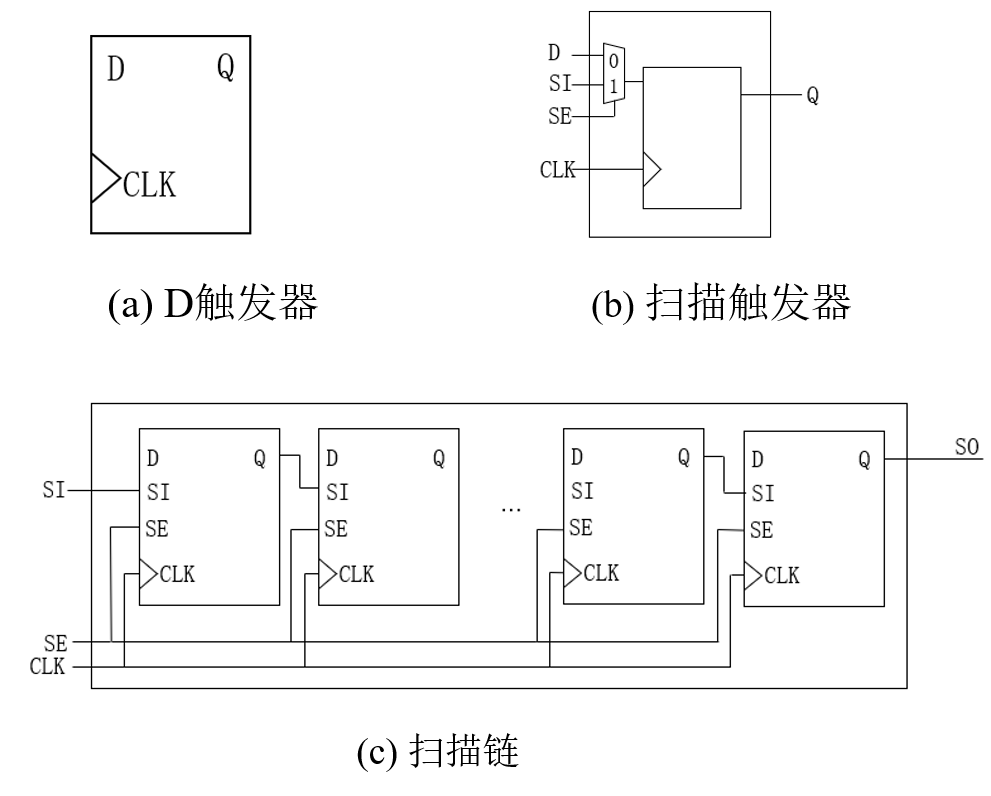
\includegraphics[width=0.5\linewidth]{assets/16/DFT扫描链.png}
  \caption{DFT扫描链}
  \label{fig:dft-scan-chain}
\end{figure}

\begin{itemize}
\tightlist
\item
  扫描链优缺点
\end{itemize}

当扫描使能信号为高时，扫描单元从扫描输入获取数据，此时扫描链构成移位寄存器，可通过扫描输入端口串行输入测试数据。在实际测试中，先将扫描使能信号端口拉高，经扫描输入端口进行测试数据移位输入；再拉低扫描使能信号端口，此时扫描单元的输入与输出均为电路中的组合逻辑，移位输入的值进入组合逻辑完成赋值并运算，在功能端口实现电路输出；之后再次拉高扫描使能信号，此时电路组合逻辑内部节点的运算结果进入扫描单元，通过移位串行输出内部节点值，以便与预期值比较，判断电路内部是否故障。扫描输入和预期输出值通常由工具自动生成，在测试向量自动生成流程中完成。

扫描链可将难以测试的时序逻辑电路转化为易测的组合逻辑电路，能有效提高电路的可测试性与可观察性，但会增加额外硬件面积，一定程度上提升了设计复杂性。

\subsubsection{测试向量自动生成}\label{sec:16-chip-frontend-030}

\begin{itemize}
\tightlist
\item
  ATPG原因
\end{itemize}

测试向量自动生成（ATPG）通过抽象电路故障模型，运用推导算法得出测试向量。现代数字系统发展迅速，测试难度大，其自动化测试数据也纳入自动化流程。借助
EDA 算法和计算机技术，自动化测试数据产生工具简化测试流程，现代 EDA
工具抽象故障、运用算法高效产生测试数据，与其他 EDA
工具配合构建全流程自动化测试体系。

\begin{itemize}
\tightlist
\item
  电路故障模型
\end{itemize}

电路故障模型主要有固定型故障、开 /
短路故障、传输延时故障等。固定型故障是目前主要且最早使用的故障类型，指电路某点信号锁定在
0 或 1
状态致电路错误，可检测大部分工艺失效，其不同位置的信号锁定在特殊情况下可等效，故在等效故障集合中选一个进行测试向量推导即可。固定开
/ 短路故障是电路中某晶体管状态固定致电路错误。传输延时故障指电路中某点
01
翻转过慢或某路径延迟过大，可能致电路时序出错，检测时需先通过一条测试向量将故障点置
0 或 1，再用另一条向量置相反值以检测节点能否在相应时间内完成翻转。

\begin{itemize}
\tightlist
\item
  测试向量中的推导算法
\end{itemize}

对电路各类故障类型抽象后，可采用不同算法推导测试向量。其中经典的 D
算法主要有几个步骤：首先是传播，确定检测某处故障后，将故障影响向输出端传递以推导期望输出；为激活故障需进行合理化，即推导其他节点的值；合理化过程中若节点值发生冲突，则需回溯至上一节点进行推导。现代各种测试向量算法多是
D 算法的优化和迭代。现代 EDA 工具可较快完成 ATPG
过程，在软件层面推导测试向量。由 ATPG 得到测试向量后，可使用
ATE（自动化测试设备）对芯片进行检测。

\begin{itemize}
\tightlist
\item
  ATPG优势以及一般要求
\end{itemize}

ATPG 优势明显。在现代 EDA
工具助力下，流程自动快捷，可大幅减少测试向量集，以最小成本实现最大测试效率。完成测试向量推导后，用故障覆盖率指标评判质量。测试覆盖率是扫描测试重要指标，由可检测故障数与故障总数比值计算，反映对设计故障的覆盖情况。一般设计的
ATPG 测试覆盖率要达 90\% 以上，航天、自动驾驶等领域要求更高，需达 99\%。

\subsubsection{自动化测试设备}\label{sec:16-chip-frontend-031}

自动化测试设备（ATE）是高度发达的测试系统，由软件系统和硬件系统组成。硬件系统包含测试通道（对应不同存储深度且有各自测试图形发生器）、时钟单元及
PCI
接口用于数据交换；软件系统包括测试图形编辑单元、设计工程接口及待测电路接口。

ATE
价格昂贵，由测试时间和总线位宽决定，时间越长、位宽越大，成本越高。为减少成本，常对多个芯片并行测试。随芯片复杂程度增高，测试图形复杂庞大，ATE
机台可能需多次加载完成测试图形载入，导致测试时间长、成本飙升，故需减小测试向量数目和大小，现代
EDA 工具一般通过压缩扫描链实现此目的。

\subsubsection{扫描链压缩}\label{sec:16-chip-frontend-032}

\begin{itemize}
\item
  压缩的重要性：扫描链压缩是在设计规模较大、扫描单元数量过多时采取的策略。若扫描链长度过大，会导致测试向量过大，可能超出
  ATE
  机台存储容量，需多次加载，增加测试时间；若减少扫描链长度，则数量增多，需较多额外端口作为测试端口，加大端口分配压力，甚至可能超过
  ATE
  机台限度，使芯片无法正常测试。因此，扫描链压缩对设计规模大、扫描单元数量多的情况意义重大。本文对加入的扫描链进行了压缩操作。
\item
  压缩原理：扫描链压缩在扫描链输入和输出端口增加额外逻辑，对测试向量进行压缩和解压缩。不同现代
  EDA 工具方式不同，如 Synopsys
  旗下工具解压缩逻辑是可编程广播式传播，压缩逻辑是异或树；Mentor
  旗下工具解压缩逻辑是环形测试向量生成器，压缩逻辑基于片上多输入签名寄存器。虽实现方式不同，但都能有效压缩测试向量，减少测试成本。扫描测试系统时钟由片上时钟控制器控制。
\item
  扫描链压缩优缺点：扫描链压缩可以有效解决设计规模较大导致扫描链数目和长度难以权衡的问题，代价是需要增加额外的逻辑，占用了额外的面积，但是在可以接收的范围内，因此扫描链压缩广泛使用在扫描测试中。
\end{itemize}

\subsubsection{片上时钟控制器}\label{sec:16-chip-frontend-033}

片上时钟控制器（OCC）在扫描测试中用于控制测试时钟。芯片处于功能模式时，OCC
输出内部时钟；处于测试模式时，输出来自 ATE
机台的慢速测试时钟，并可旁路内部时钟，实现功能模式与测试模式切换。若不选择测试时钟，测试机台对测试过程可控性下降且易受内部时钟干扰，问题难定位。加入
OCC 后，ATPG 工具能更有效追踪扫描链。OCC 一般位于 PLL 之后，输入 PLL
生成的快速时钟和 ATE
的慢速时钟，在不同模式下由控制信号选通不同时钟源。加入 OCC
后会生成时钟链，与扫描链不同，OCC
需要额外端口控制，会带来一定测试端口和电路面积开销。

\subsection{内建自测试}\label{sec:16-chip-frontend-034}

内建自测试（Built In Self
Test，BIST）是在芯片内部自动测试的技术，存储器的故障模式相对较为明确，且对存储器进行全面测试较为困难，所以内建自测试在存储器测试中广泛应用。存储器内建自测试（Memory
Built-in Self
Test，MBIST）即在存储芯片内部引入测试向量生成模块和测试向量检测及压缩模块，可以有效对电路内部的缺陷进行检测，不依赖于昂贵的ATE设备，如图\ref{fig:MBIST}。

\begin{figure}[htbp]
  \centering
  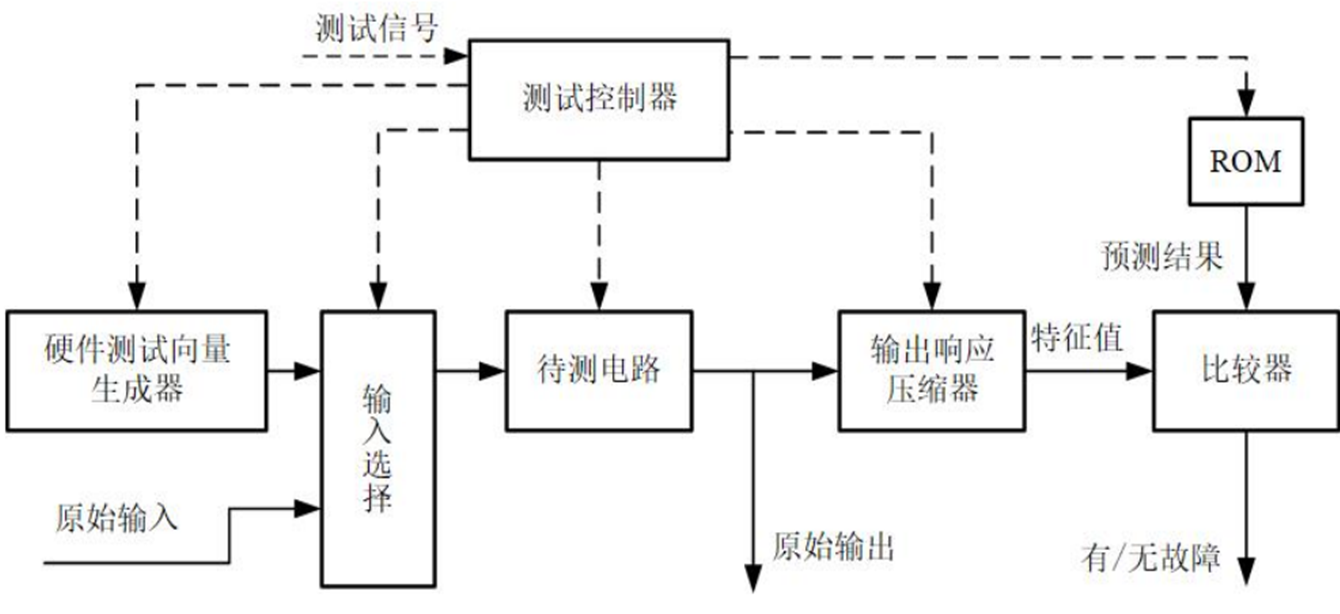
\includegraphics[width=0.5\linewidth]{assets/16/内建自测试电路模块示意图.png}
  \caption{内建自测试模块示意图}
  \label{fig:MBIST}
\end{figure}

\subsubsection{存储器故障类型}\label{sec:16-chip-frontend-035}

存储器主要包括地址解码，存储和读写控制单元，主要故障类型包括单元固定故障，状态跳变故障，单元耦合故障等类型。单元固定故障，即Stuck
At Fault，是指存储器单元固定在0或者1状态；状态跳变故障，即Transition
Delay
Fault，是指对存储器进行读写操作时，存储器状态跳变异常；单元耦合故障是，即Coupling
Fault，指当存储器单元发生状态跳变时，会对其周围存储器单元造成影响，该种故障类型主要针对RAM。针对不同类型的故障，需要不同的测试激励进行检测。例如要检测单元固定故障，则需要对可能存在故障的单元进行数据0/1的读写。

\subsubsection{存储器测试算法}\label{sec:16-chip-frontend-036}

对存储器的测试算法主要包括棋盘式图形算法和March算法。其中棋盘式图形算法通过对相邻存储器进行分组，向不同组写入01交替的测试向量，之后对存储器进行读取操作，可以检测某些存储器故障。March算法在目前广泛使用，对不同单元进行依次操作，March算法中的操作单元称为March单元，由各种不同的操作序列组成，March算法有不同变体，对故障类型的覆盖各有差异，覆盖率也有所不同。
